\documentclass[a4paper,11pt,dvipdfmx]{jsarticle}

\usepackage{bm}
\usepackage[dvipdfmx]{graphicx}
\usepackage[dvipdfmx]{color}
\usepackage[subrefformat=parens]{subcaption}
\usepackage{ascmac}
\usepackage{siunitx}
\usepackage{otf}
\pagestyle{plain}
\usepackage{float}
\usepackage[dvipdfmx]{hyperref}
\usepackage{pxjahyper}
\usepackage{here}
\usepackage{titlesec}
\titleformat*{\section}{\LARGE\bfseries}
\titleformat*{\subsection}{\normalsize\bfseries}
\usepackage{url}
\usepackage[table,xcdraw]{xcolor}
\hypersetup{% hyperrefオプションリスト
setpagesize=false,
 bookmarksnumbered=true,%
 bookmarksopen=true,%
 colorlinks=true,%
 linkcolor=blue,
 citecolor=blue,
}


\begin{document}
\newpage
\section{\LARGE{データ収集と解析(担当:金\UTF{FA11})}}

\subsection{DAQ systemの構築}
本節ではDAQ system(Data AcQuition system:データ収集系)について述べる。本研究ではターゲット原子核へ陽子を入射し、散乱後の粒子のエネルギースペクトルを得ることで、散乱断面積を求める。検出器であるPINフォトダイオードの出力信号の波高から、スペクトルを得るためのDAQ systemの構築を目指した。
\subsubsection{手段の検討}
昨年度のラザフォード散乱実験\cite{2019}では波高データの読み出しにはMCA(Multi Channel Analyzer)を使用していた。以下にその検出回路を示す。

\vspace*{5mm}

\begin{figure}[H]
\centering
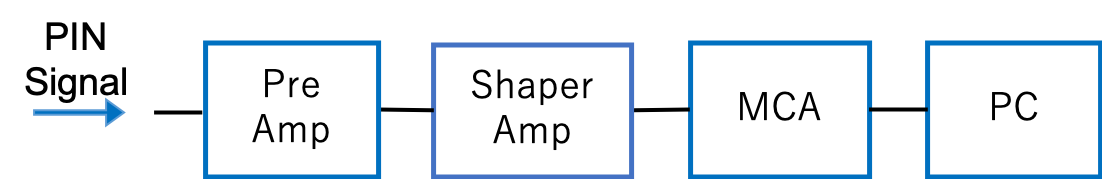
\includegraphics[width=100mm]{picture/daq/MCA.png}
%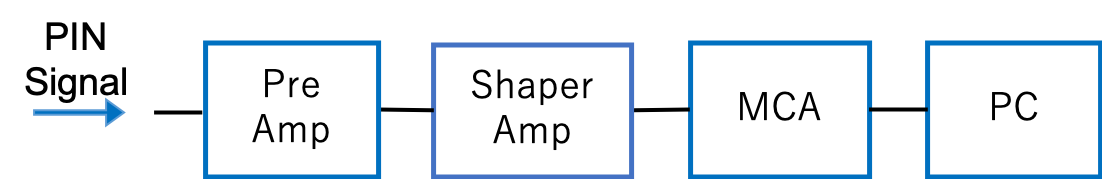
\includegraphics[bb=0 0 1102 179,width=100mm]{picture/daq/MCA.png}
\caption{MCAを用いた検出回路}
\label{MCA}
\end{figure}

\vspace*{5mm}

本年度の新たな試みとして、p-p散乱の観測を目指したことが挙げられる。昨年度使用していたMCAでは、同じ散乱イベント由来の波高データを時間同期しながら得ることができなかった。そこでVME busモジュールを用いた2ch同時計測回路の構築を行うこととした。

\subsubsection{VME bus}
VME bus(Versa Module Eurocard bus)とは1981年に開発されたコンピュータのバス規格の一つである。同じく高エネルギー物理学実験などに用いられるCAMAC 規格と比べてデータ転送が速いという特徴を持つ。VMEクレートに挿入されたモジュールはバックブレーンを介してデータの通信を行う。本研究ではピークホールド型のADCと、SiTCP VME Masterの2つのモジュールを用いた。以下その役割や性能を述べる。

\newpage
\begin{description}
   \item[● ピークホールド型ADC]\mbox{}\\
   ADC(Analog-to-Digital Converter)とはアナログ信号をデジタル値に変換するシステムである。信号の波高分布を得るため、本研究ではピークホールド型のADC(以降PHADC)を用いた。PHADCのGate入力端子に信号が与えられている間のピーク電圧をデジタル変換する。\\

   \item[● SiTCP VME Master]\mbox{}\\
   Eathernet経由でVME busを制御するためのMaster Moduleである。同一のクレートに挿入されている VME Slave Moduleへのアクセスが可能。PHADCの制御・データ読み出しに用いた。
   
\vspace*{5mm}
   
 \begin{figure}[H]
    \begin{tabular}{cc}
      \begin{minipage}[t]{0.45\hsize}
        \centering
        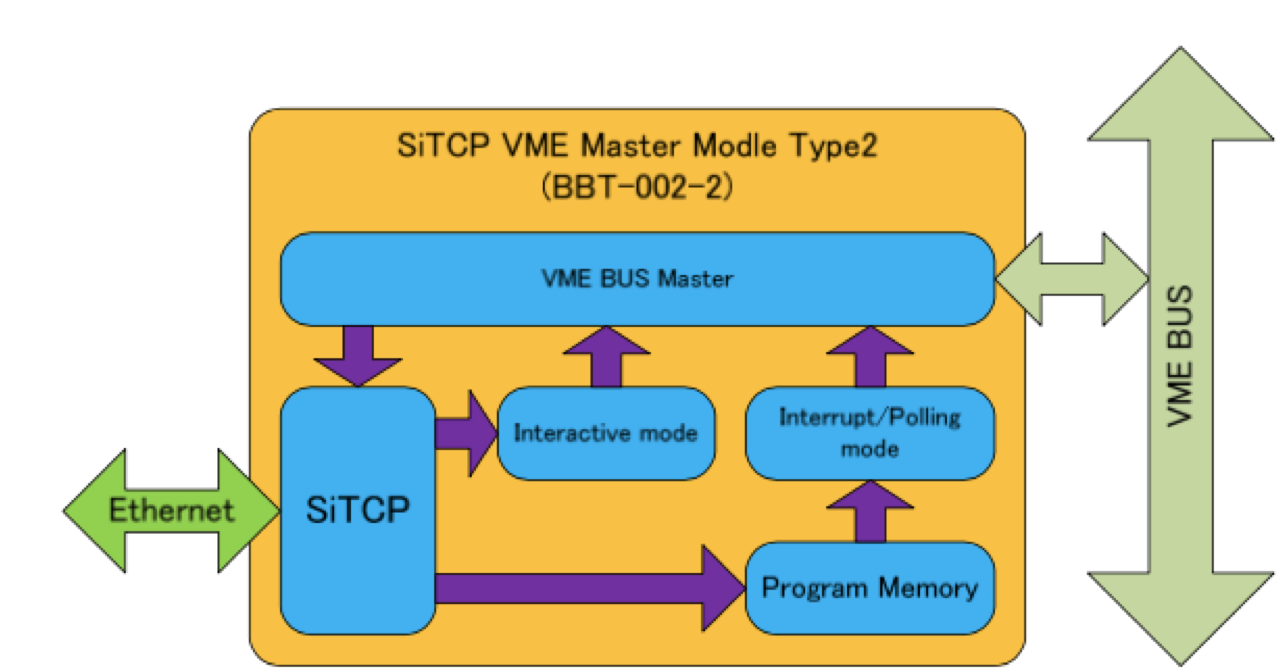
\includegraphics[width=62mm,height=50mm]{picture/daq/SiTCP.png}
        \caption{SiTCP 全体ブロック図\cite{BBT}}
        \label{SiTCP1}
      \end{minipage} &
      \begin{minipage}[t]{0.45\hsize}
        \centering
        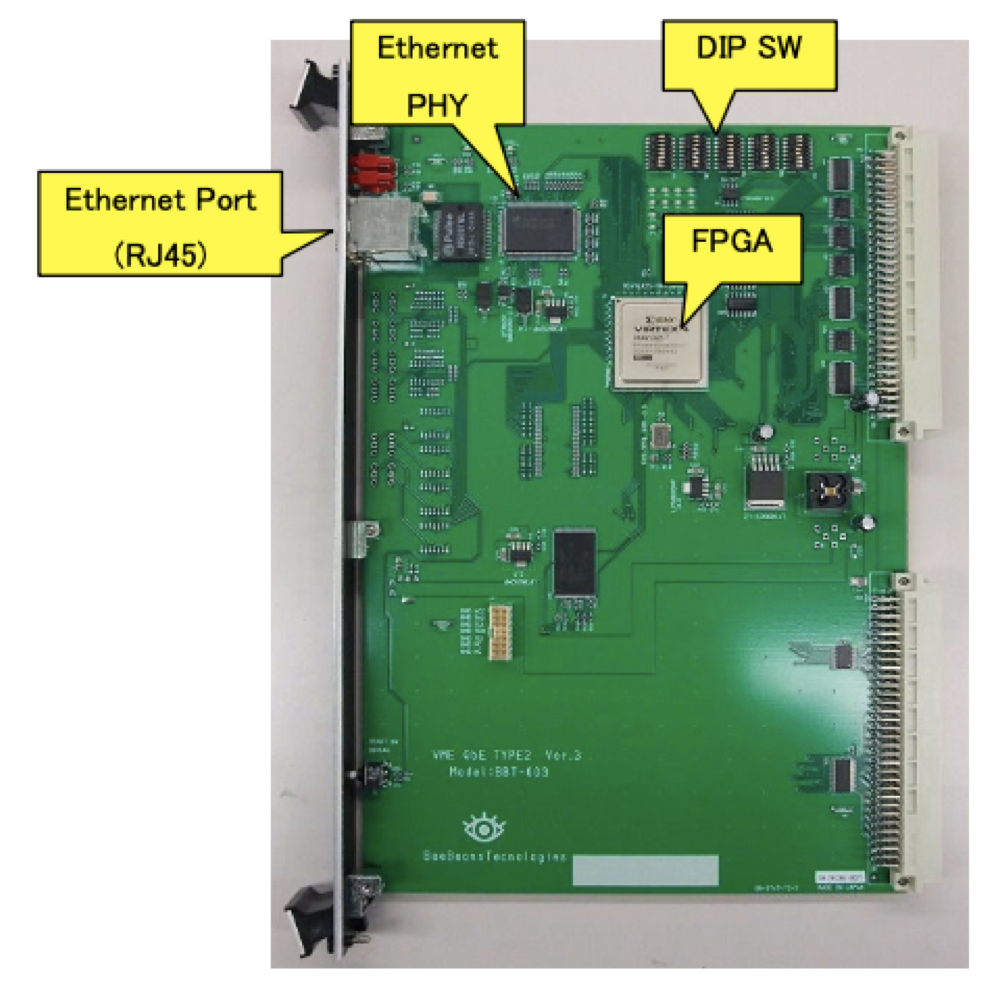
\includegraphics[width=64mm,height=70mm]{picture/daq/SiTCP2.png}
        \caption{SiTCP 全体写真\cite{BBT}}
        \label{SiTCP2}
      \end{minipage}
    \end{tabular}
  \end{figure}
  
\end{description}

\vspace*{5mm}

\begin{table}[h]
   \caption{使用したVMEモジュール\cite{BBT}\cite{hoshin}}
   \centering
   
  \begin{tabular}{ccc} \hline
  モジュール名 & 制作元:型番 & スペック等 \\ \hline \hline
  PHADC & 豊伸電子:8ch PHADC V006 & 
  \begin{tabular}{c}
    最大入力:4V\\
    逐次14bit変換\\
    入力インピーダンス:1k$\Omega$ \\
    最小Gate幅:500ns
   \end{tabular} \\ \hline
    SiTCP VME Master & BeeBeansTechnologies:BBT-002-2 &
    \begin{tabular}{c}
    通信プロトコル:TCP
   \end{tabular} \\ \hline

  \end{tabular}
  \centering
\end{table}

\newpage
\subsubsection{2ch同時計測回路の構築}
前節で述べたように、PHADCにはTrigger信号としてGate入力を与える必要がある。入射陽子と反跳水素原子核は、散乱イベント発生からおよそ同じ時間で検出器に到達すると予想される。(散乱後の二粒子のエネルギー差を考慮した理論的な到達時間の最大差 < 10ns )。したがって2つの信号を同時計数回路(コインシデンス)へ入力すれば、適切なタイミングでTriggerをかけることができると考えた。以下に2ch同時計測回路のブロック図[図\ref{coin}]と使用したNIMモジュール[表\ref{NIM}]を示す。ルーターにはbuffalo社のWSR-1800AX4-BKを用いた。

\vspace*{7mm}

\begin{figure}[H]
\centering
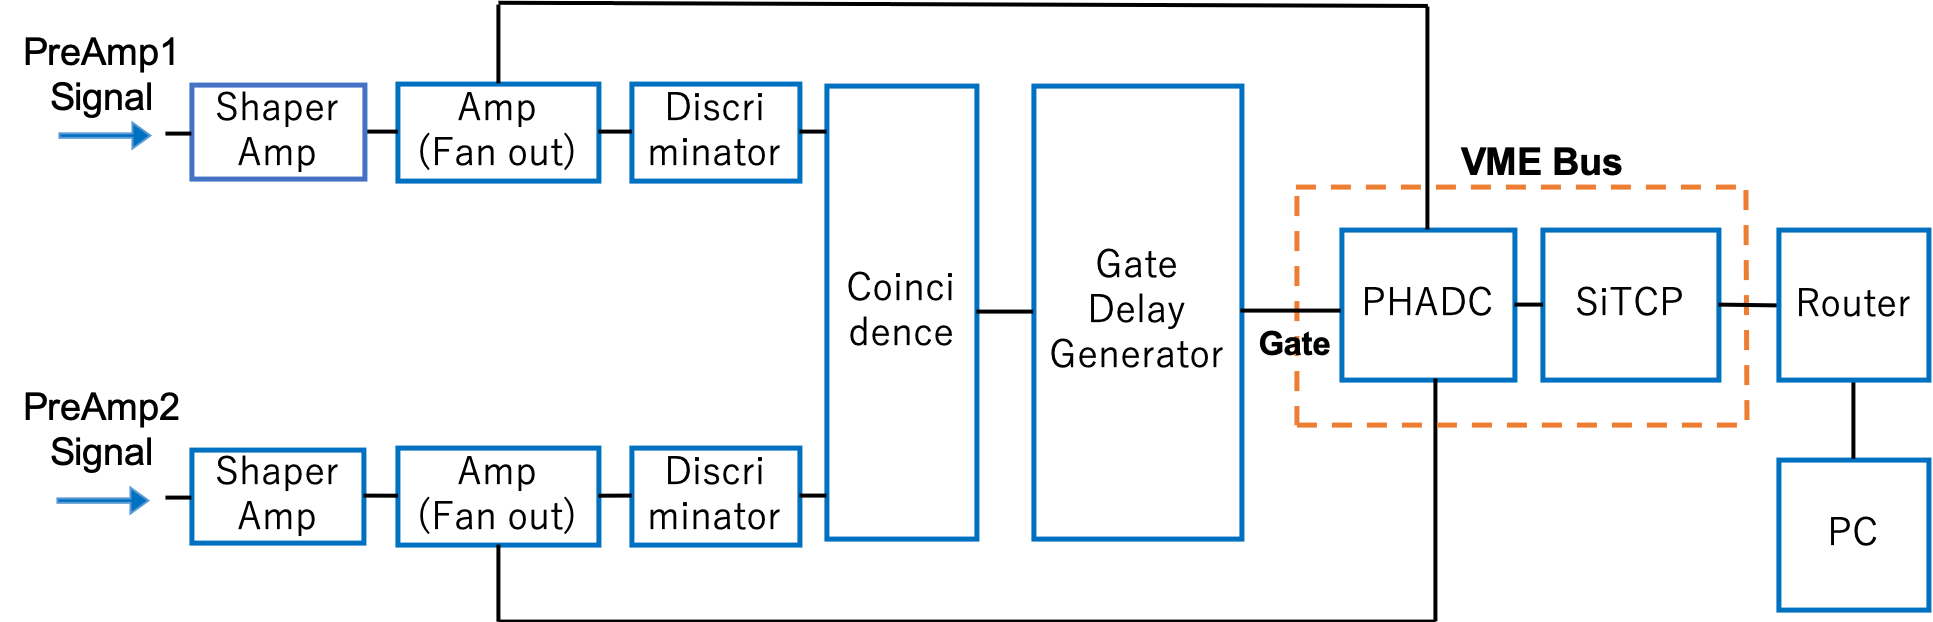
\includegraphics[width=150mm,height=60mm]{picture/daq/PHADC.png}
\caption{2ch同時計測回路}
\label{coin}
\end{figure}

\vspace*{5mm}

\begin{table}[h]
   \caption{使用したNIMモジュール\cite{hoshin}\cite{repic}}
   \centering
   
\begin{tabular}{ccc} \hline
  モジュール名 & 制作元:型番 & スペック、実験時の設定等 \\ \hline \hline
  アンプ & 豊伸電子:N018 & 出力gain:10 \\ \hline
  コインシデンス & 豊伸電子:N017 & 
  \begin{tabular}{c}
    応答速度:2ns~ \\
    アナログ加算式(ANY1$\sim$4)
   \end{tabular} \\ \hline
    ゲートジェネレーター & 豊伸電子:N014 & Gate幅:約1$\mu$s \\ \hline
    ディスクリミネーター & ハヤシレピック:RPN-110 & 最小Threshold:-20mV \\ \hline
    シェーパーアンプ & 豊伸電子:N012 &
    \begin{tabular}{c}
    時定数:0.15$\mu$s \\
    出力gain:ADC$\rightarrow$10、MCA$\rightarrow$20
    \end{tabular} \\ \hline
  \label{NIM}
  \end{tabular}
  \centering
\end{table}

\newpage
\subsubsection{Trigger Logic}\label{logic}
ここではTriggerシステムについて述べる。まずは使用したモジュールの説明を行う。\\
\begin{description}
   \item[● ディスクリミネーター(波高弁別回路)]\mbox{}\\
   Threshold電圧より大きい入力信号が与えられたとき、矩形波を出力する\\
   \item[● コインシデンス(同時計数回路)]\mbox{}\\
   4つの入力チャンネルを持つ。本論文では4つのうちいずれか1つ以上に信号が入力されたときに矩形波を出力するモードがANY1、2つ以上に入力があったときに矩形波を出力するモードをANY2と定義する。\\
   \item[● ゲートディレイジェネレーター]\mbox{}\\
   信号入力があったとき、任意の時間幅の矩形波を出力する。出力時間にディレイをかけることもできるが、本実験ではディレイ機能は用いていない。\\
\end{description}

\noindent
本実験で用いたTriggerシステムの概略を図\ref{Logic}に示す。
ディスクリミネーターにはプリアンプ・シェイパーアンプ・アンプを通した信号を入力している。この入力に対してディスクリミネーターが矩形波を出力し、2チャンネルで同時に出力されたときにコインシデンスが矩形波を出力する。その信号をゲートジェネレーターに入力することで、TriggerとなるGate信号を作成した。

\vspace*{5mm}

\begin{figure}[H]
\centering
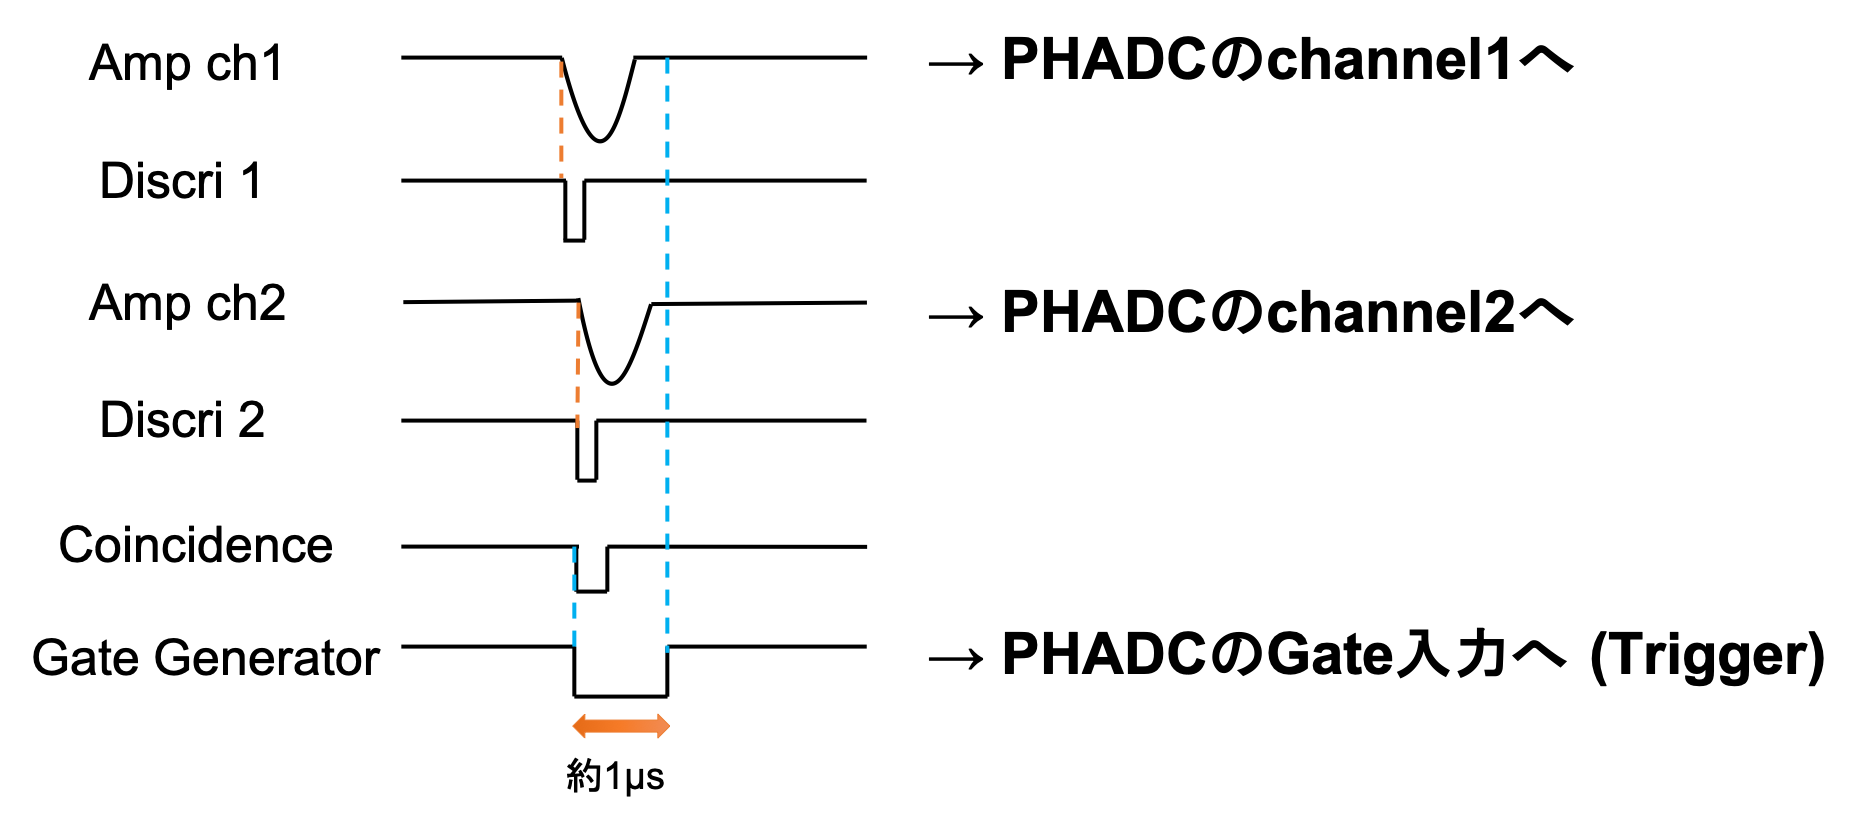
\includegraphics[width=150mm,height=65mm]{picture/daq/Trigger.png}
\caption{Trigger Logic}
\label{Logic}
\end{figure}

\newpage
\subsubsection{その他の設定}
ディスクリミネーターのThresholdは、真空チェンバー内でのノイズを拾わないレベルの電圧値で設定を行なった。パルスジェネレーターでその電圧値を確認したところ、およそ-100mVであった。

ゲートジェネレーターの出力の時間幅は、PINフォトダイオードに $\alpha$ 線($^{241}\mathrm{Am}$線源)を照射したときの信号を用いておよそ1$\mu$sに設定した。またPHADCは正負のどちらでもピーク電圧をデジタル変換するようになっているが、負の電圧に比べて正の電圧を入力した方がデータ収集が安定したため負の信号から正の信号へと変換を行なった。変換にはPulse Electronis社のPE-62245を用いた。[図\ref{Gate}]

\vspace*{5mm}

 \begin{figure}[H]
    \begin{tabular}{cc}
      \begin{minipage}[t]{0.50\hsize}
        \centering
        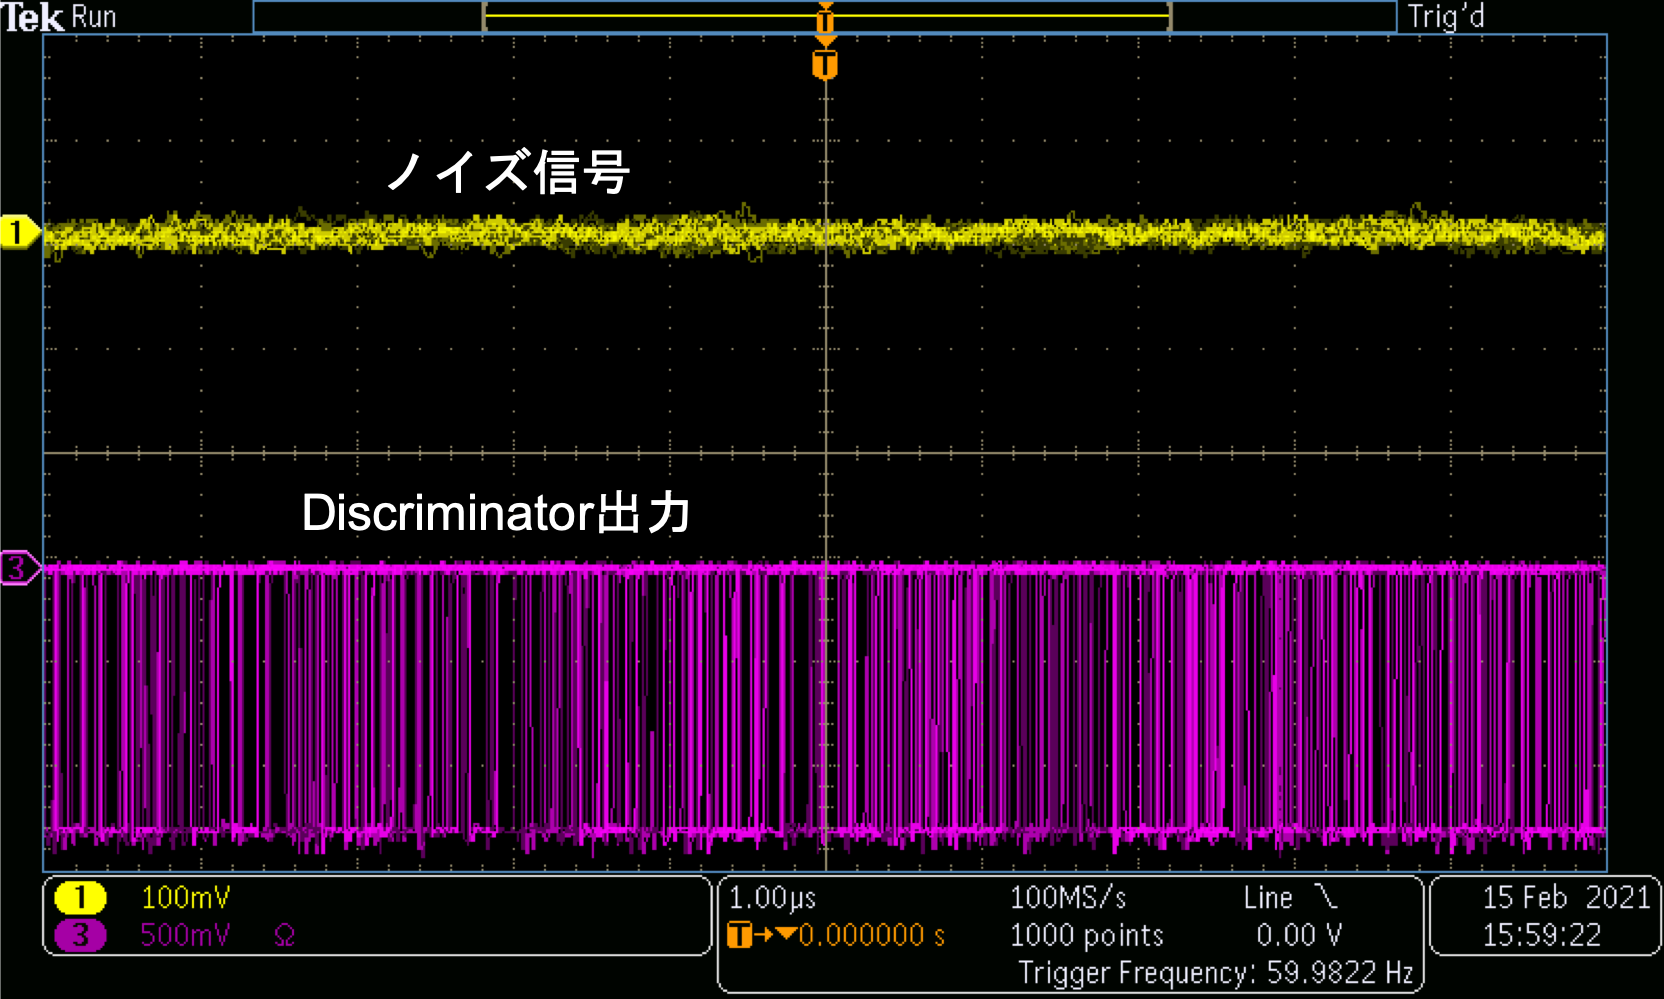
\includegraphics[width=65mm,height=42mm]{picture/daq/noise.png}
        \caption{ノイズ信号にディスクリミネーターが反応している様子}
        \label{noise}
      \end{minipage} &
      \begin{minipage}[t]{0.50\hsize}
        \centering
        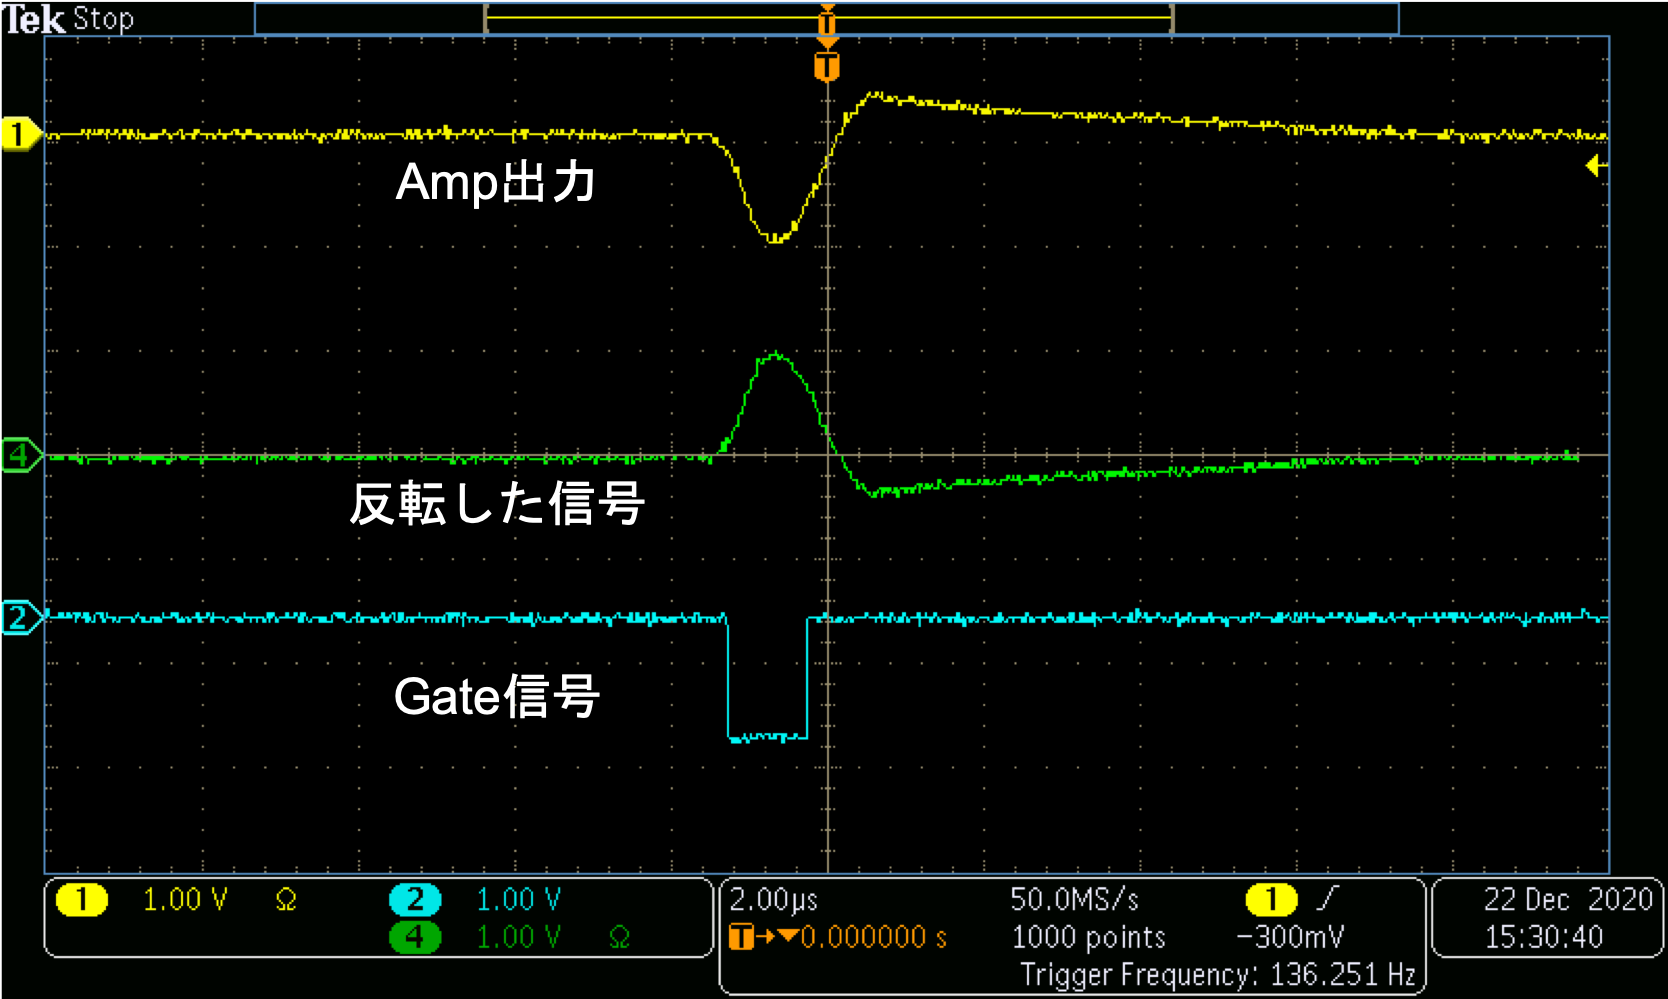
\includegraphics[width=65mm,height=42mm]{picture/daq/Gate.png}
        \caption{信号の反転とGate信号}
        \label{Gate}
      \end{minipage}
    \end{tabular}
  \end{figure}

\vspace*{3mm}

\begin{figure}[H]
\centering
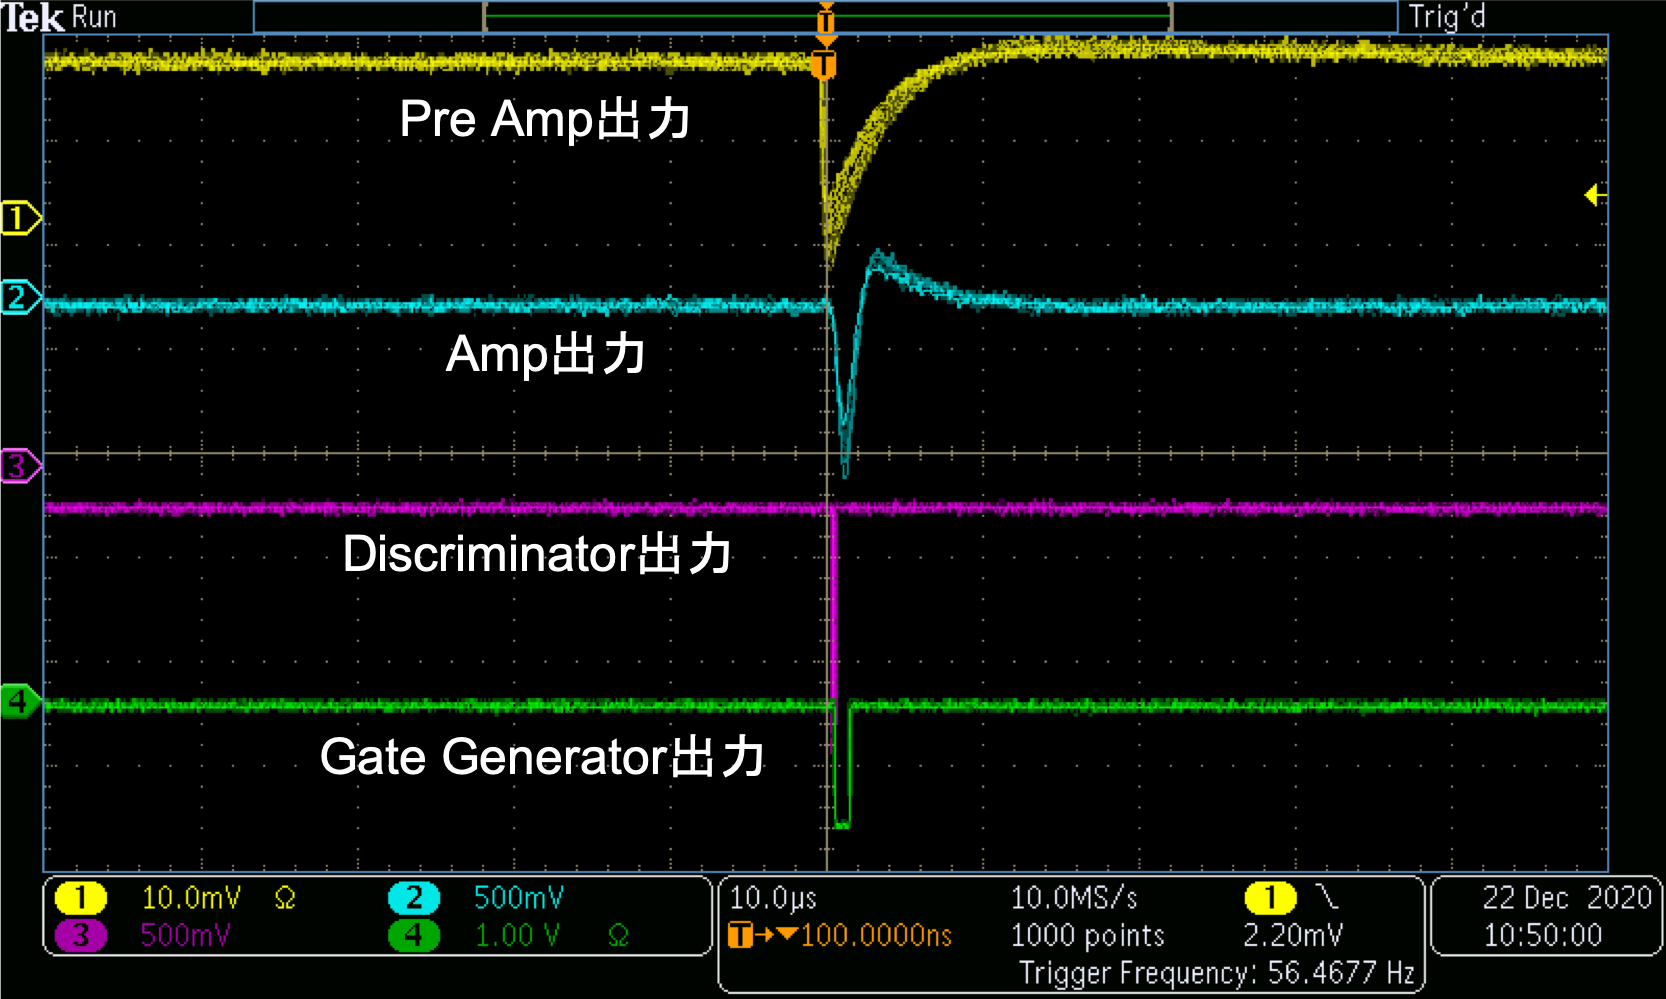
\includegraphics[width=100mm,height=60mm]{picture/daq/signal.png}
\caption{適切な各モジュールの出力}
\label{signal}
\end{figure}

\newpage
\subsection{DAQ systemの動作確認}
海事科学部での本実験の前に、DAQ systemの動作確認を行なった。確認事項としては、得られるエネルギースペクトルおよびその解析プログラム、2ch同時計測回路の動作、そしてトリガーレート等が挙げられる。本節ではその試験結果を述べる。

\subsubsection{エネルギースペクトル}
正しいエネルギースペクトルが得られているかは、PINフォトダイオードに$\alpha$ 線($^{241}\mathrm{Am}$線源)を照射することで確認した。$\alpha$線源とPINフォトダイオードとの距離を0$\sim$2cmの1cmごとに設定し、計測を行うことで空気中でのエネルギー損失の要素を含んだエネルギースペクトルが得られるかを試みた。$\alpha$線や陽子線などの重荷電粒子は物質中を透過するとき、進行方向の物質を励起しながらエネルギーを失っていく。図\ref{Bragg}に、5.49 MeVの$\alpha$線の空気中でのBragg曲線を示す。$^{241}\mathrm{Am}$線源における$\alpha$線のエネルギーは5.4 MeVであるが、エネルギー損失の過程は同様なBragg曲線 に従うと考えられる。図\ref{0to2}に得られたエネルギースペクトルを示す。距離が大きくなるにつれて、波高が小さくなっていく様子が見られる。この結果から正常に動作していると評価した。\\

%\vspace*{5mm}
\begin{figure}[H]
\centering
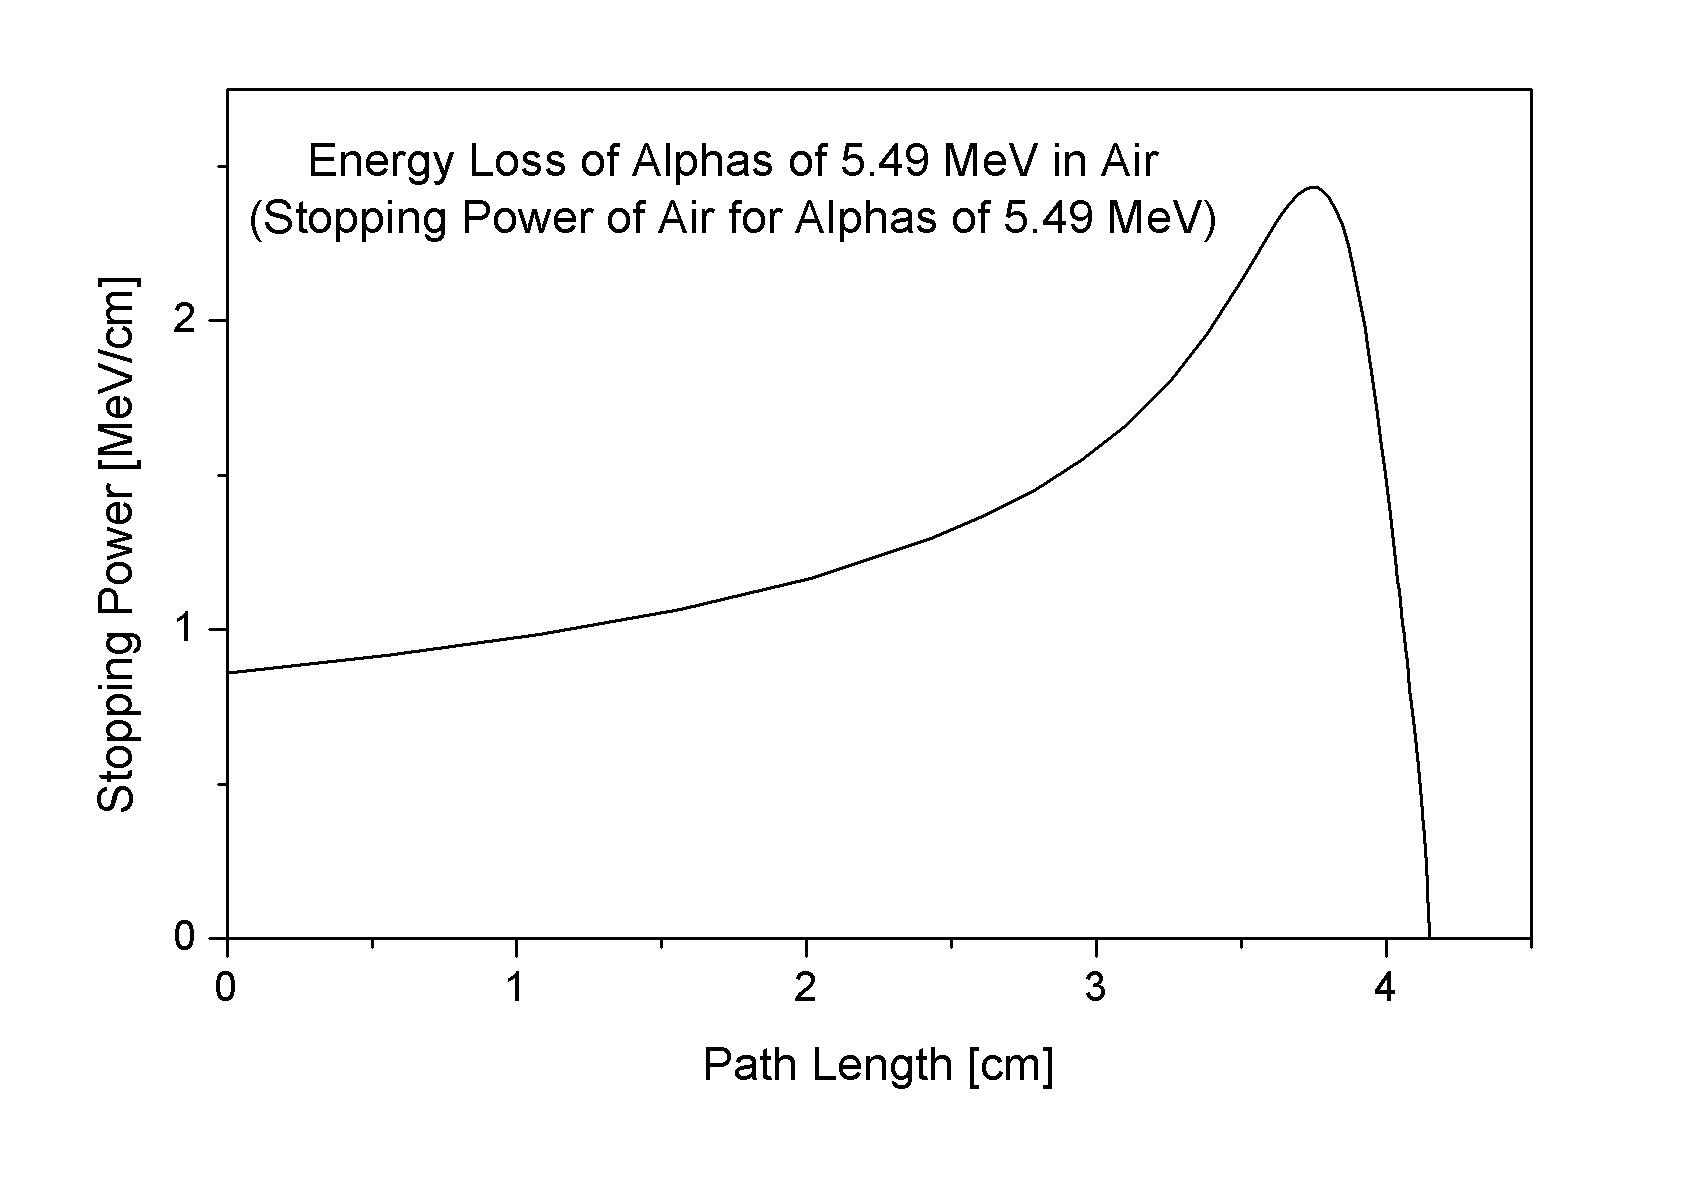
\includegraphics[width=120mm]{picture/daq/Bragg.png}
\caption{5.49 MeVの$\alpha$線に対するBragg曲線\cite{braggpeak}}
\label{Bragg}
\end{figure}

\begin{figure}[H]
\centering
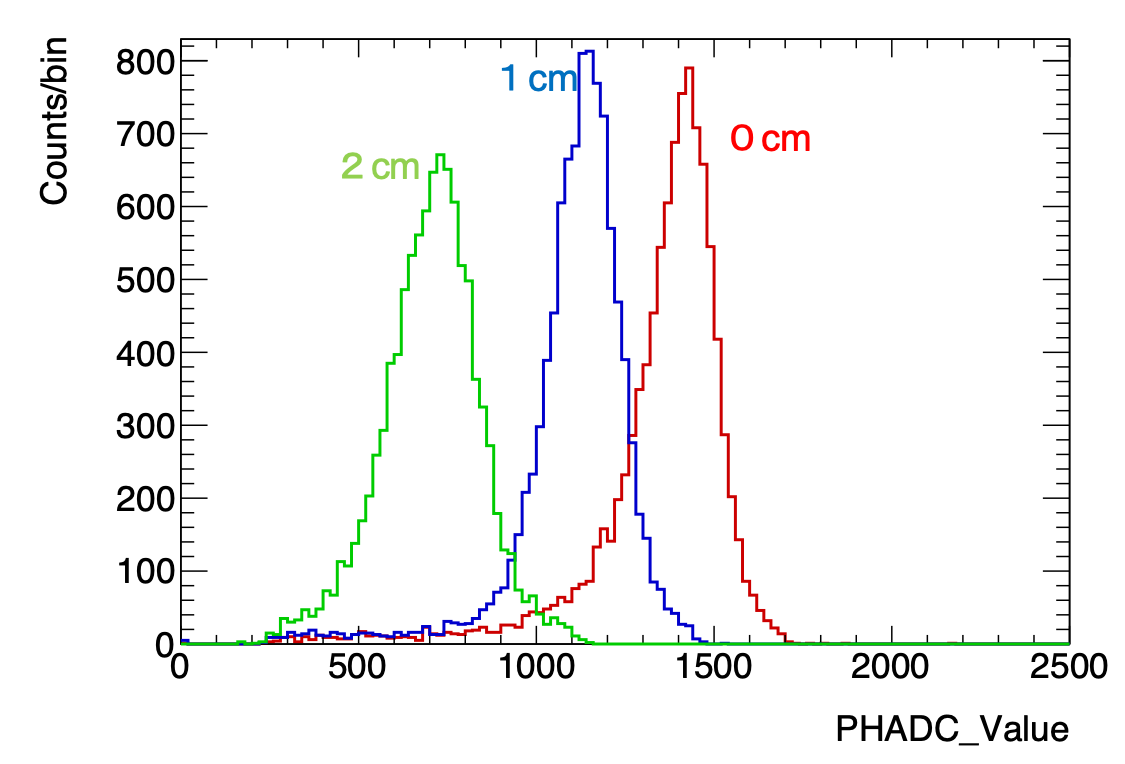
\includegraphics[width=110mm]{picture/daq/0to2cm.png}
\caption{3つの検出距離におけるエネルギースペクトル}
\label{0to2}
\end{figure}
\begin{figure}[H]
\centering
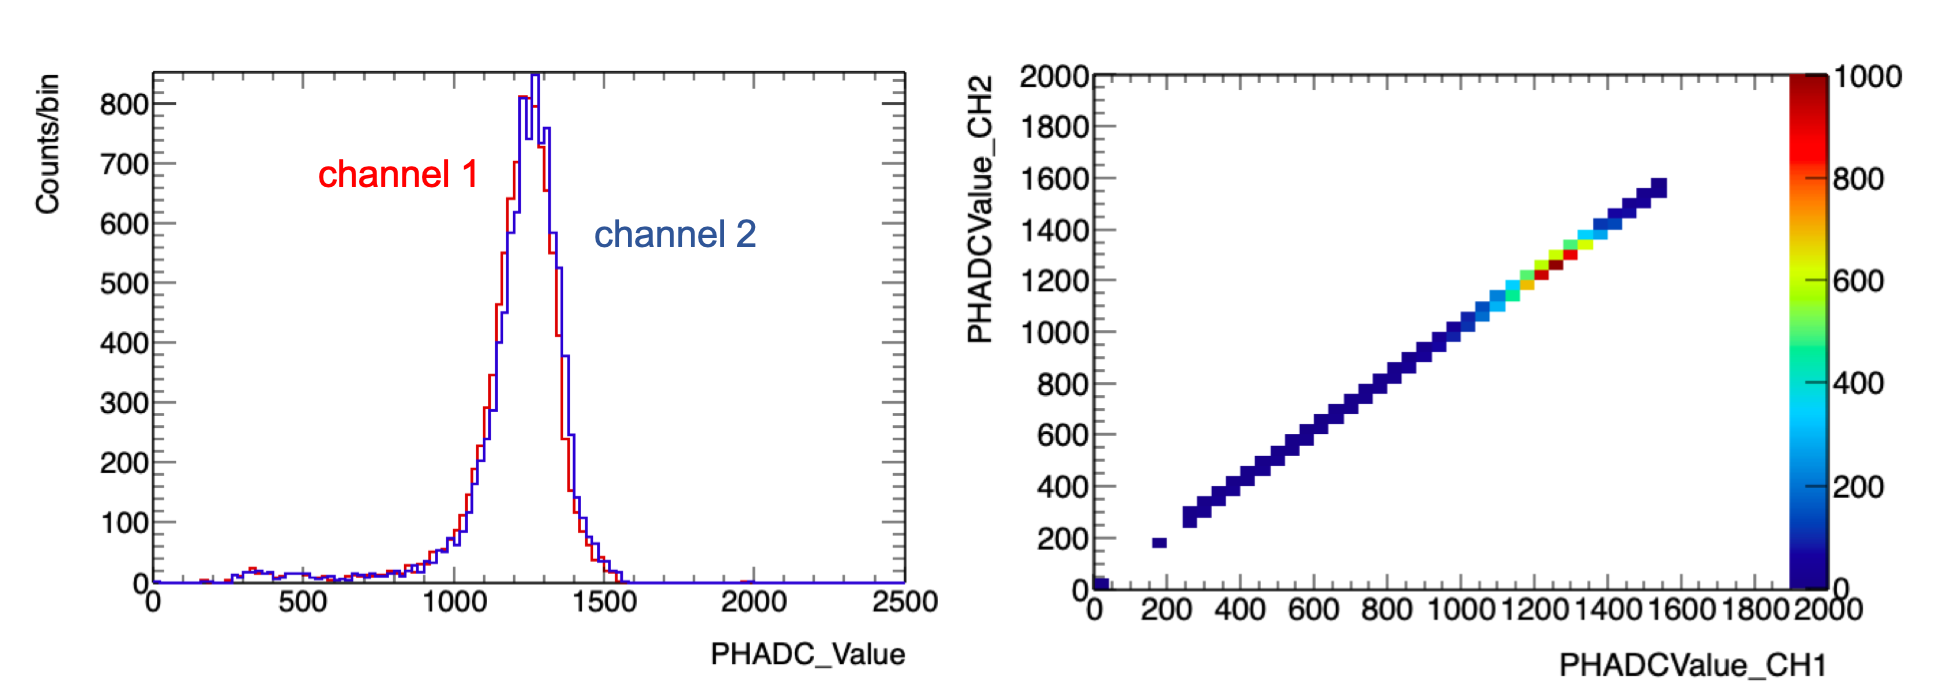
\includegraphics[width=155mm]{picture/daq/2ch.png}
\caption{2ch同時計測回路の試験結果}
\label{2ch}
\end{figure}

\subsubsection{2ch同時計測回路の確認}
2ch同時計測回路の動作確認は、$\alpha$線の信号を並列回路を用いて2つに増やしそれぞれPHADCに入力して行なった。2つのチャンネルで得られたエネルギースペクトルと二次元ヒストグラムを図\ref{2ch}に示す。

二次元ヒストグラムから、2つのチャンネルの値が等しくなっていることが分かる。この結果から2ch同時計測回路が正常に動作していると判断した。

\subsubsection{トリガーレートの考慮}
強い陽子ビームを照射すると、高いレートでトリガーがかかることが予想される。そこで事前にトリガーレートの上限値を検証する必要があった。PHADCのGate入力に、パルスジェネレーターを用いて指定したレートでパルスを入力し、1000イベント計測終了までの時間を記録し理論値との比較を行った。[図\ref{trigger}]

理論上では計測にかかる時間はパルスのレートと反比例の関係にあるが、図\ref{trigger}にあるように、1ch計測回路では90Hz、2ch同時計測回路では70Hzあたりを境に計測時間は理論の値よりも大きくなっている。

\begin{figure}[H]
\centering
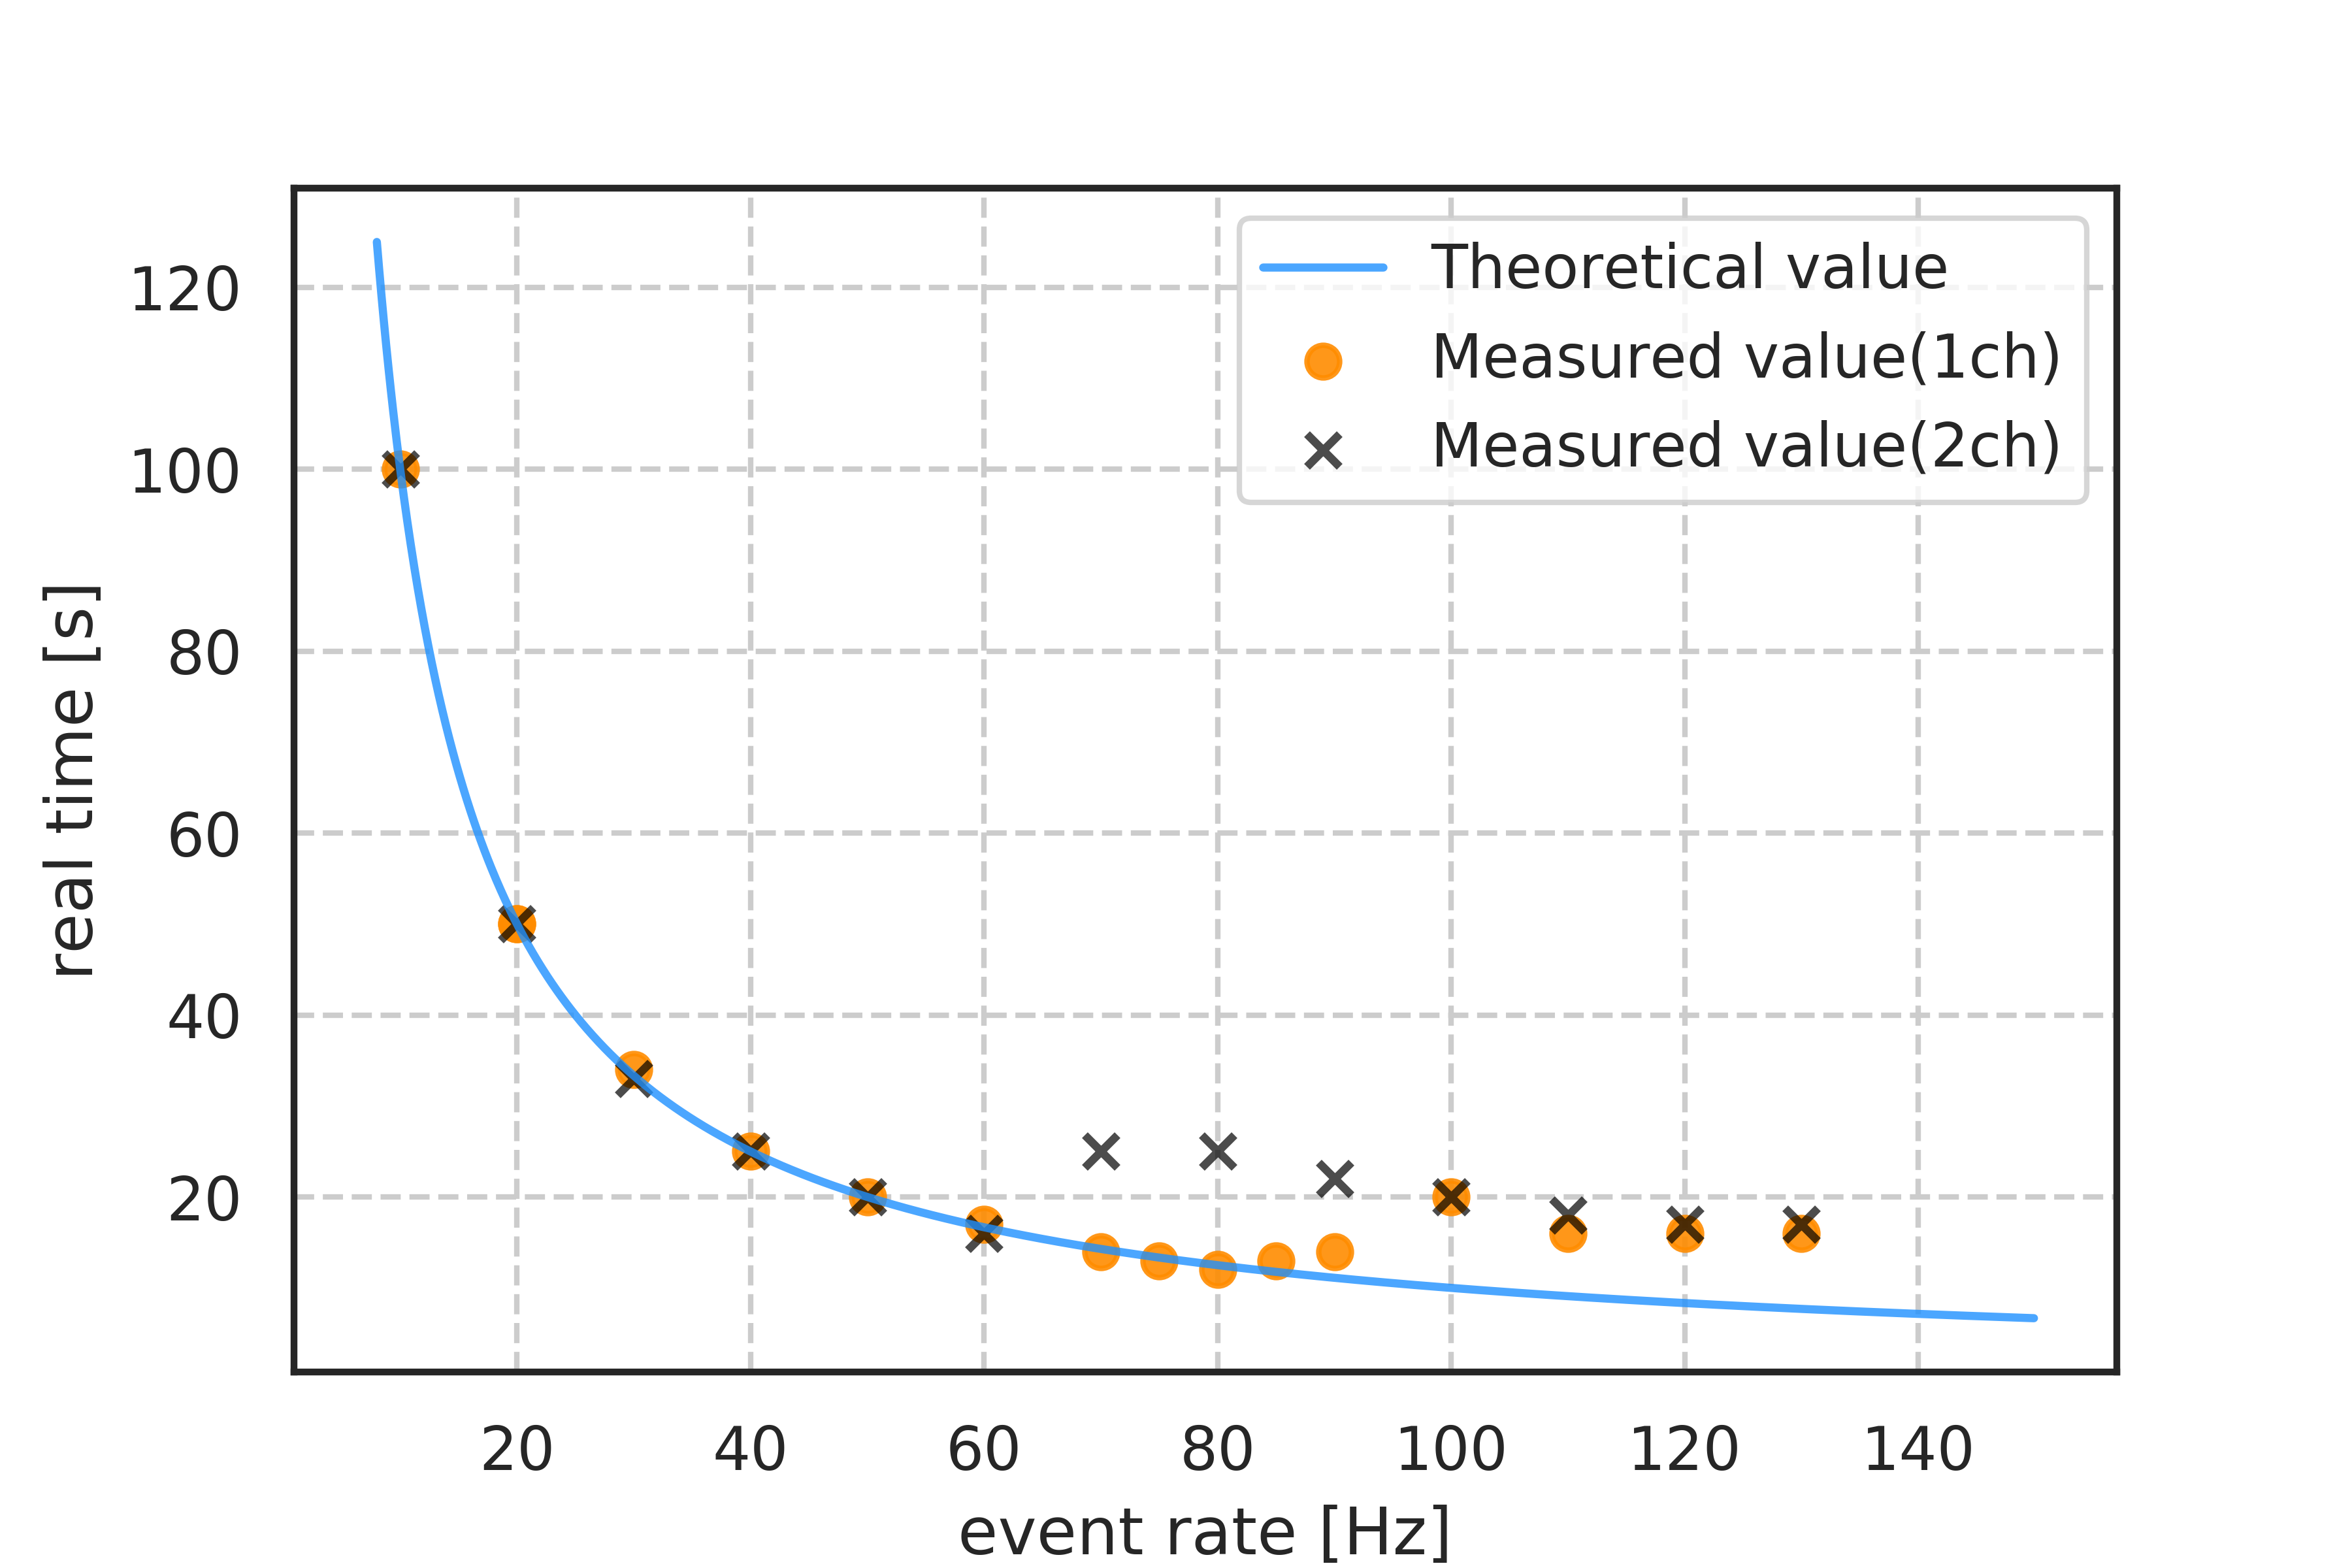
\includegraphics[width=120mm]{picture/daq/trigger_test.png}
\caption{トリガーレートの検証}
\label{trigger}
\end{figure}

\vspace*{5mm}
\noindent
炭素原子核を標的とした場合の、散乱角$40^\circ$における散乱陽子の検出器への入射レートを\eqref{eq:expcs}式を用いて求めた。[表\ref{Rate}]

\begin{table}[h]
   \caption{散乱陽子の予想入射レート}
   \centering
   
\begin{tabular}{cc} \hline
  電流値 [nA] &入射レート [Hz] \\ \hline
  
  \begin{tabular}{c}
    0.1  \\
    1 \\
    10 \\
    100 \\
   \end{tabular} &
   
     \begin{tabular}{c}
    42 \\
    4.2$\times$${10}^2$ \\
    4.2$\times$${10}^3$ \\
    4.2$\times$${10}^4$ \\
   \end{tabular} 
   \\ \hline
   \end{tabular}
   \label{Rate}
\end{table}

\vspace*{5mm}

以上から、電流値の設定や散乱角によっては100Hzを超えるレートでトリガーがかかると予想される。散乱断面積の値を求めるには散乱された粒子の数を正確に求める必要があること、コインシデンスを取る必要がないことから、散乱断面積を求めるための計測にはMCAを用いることとした。MCAはAMP TEK社のMCA8000D(最大トリガーレート:100 MHz)を使用した。

\vspace*{15mm}

\begin{figure}[H]
\centering
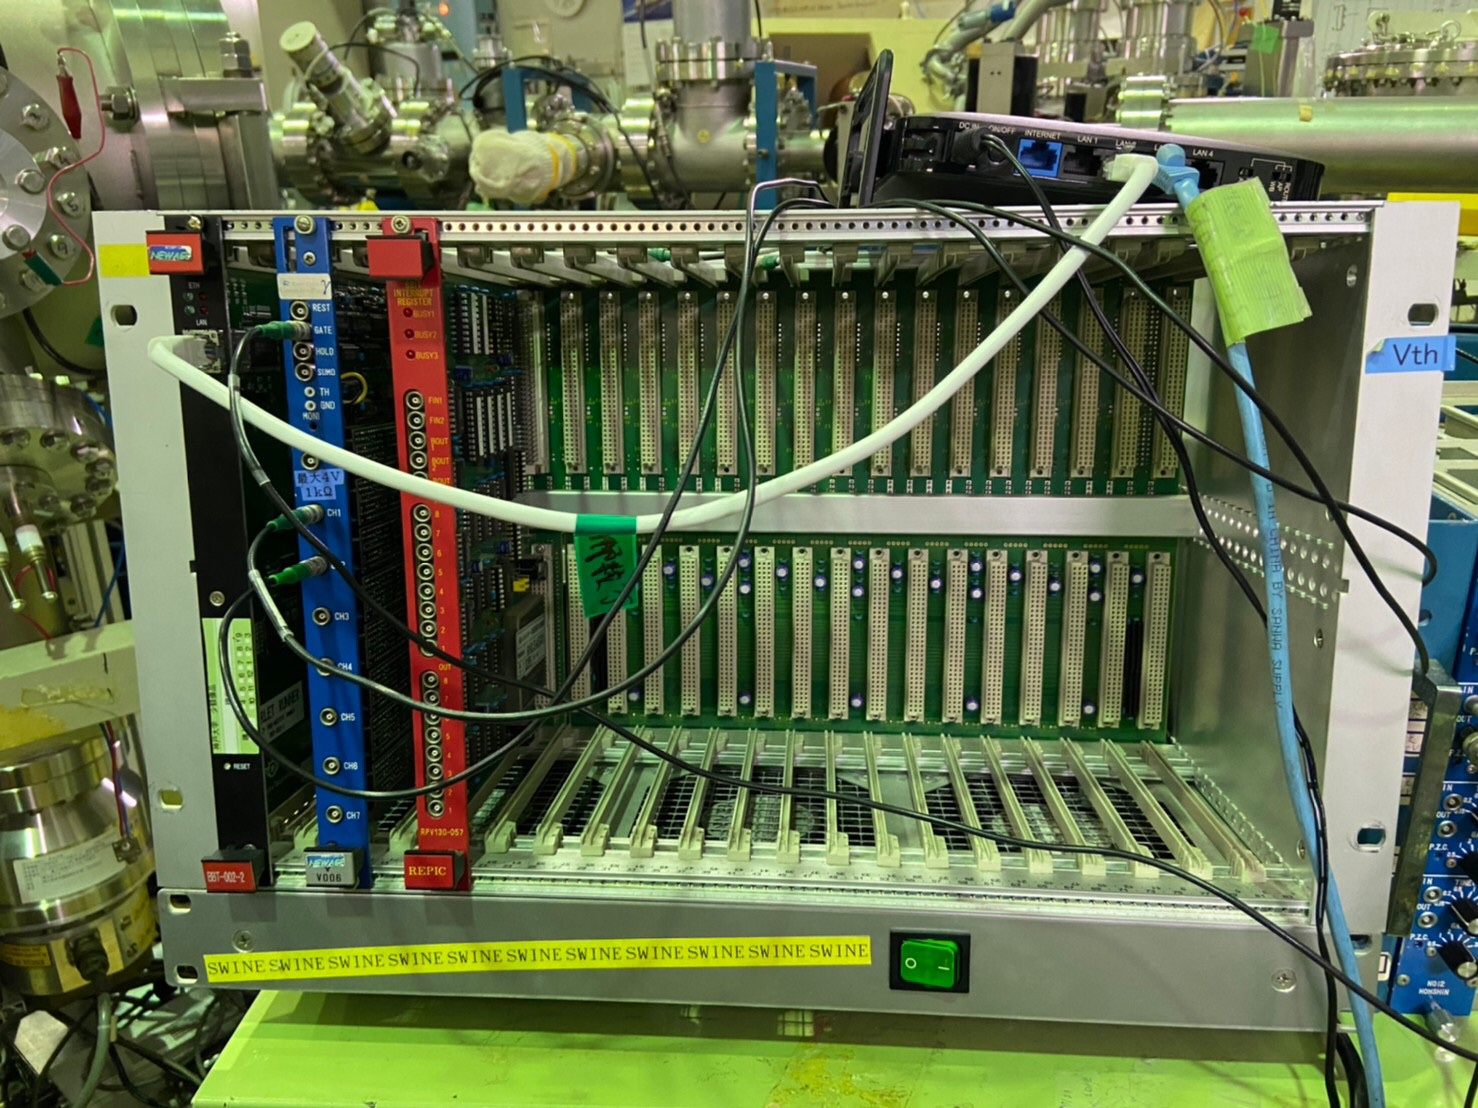
\includegraphics[width=120mm]{picture/daq/vme.JPG}
\caption{使用したVMEクレートとモジュール}
\label{vme}
\end{figure}

\newpage



\end{document}